\chapter{Қаңқалы дарақ}

\index{қаңқалы дарақ}


{Қаңқалы дарақ} 
графтың барлық төбелерінен және кез келген екі төбесі арқылы жол болатындай  қырлар ішжиынынан тұрады.
Олар да жалпы дарақ сияқты ациклді және байланысқан болады.
Әдетте қаңқалы дарақты құрудың бірнеше тәсілі болады.
% A \key{spanning tree} of a graph consists of
% all nodes of the graph and some of the
% edges of the graph so that there is a path
% between any two nodes.
% Like trees in general, spanning trees are
% connected and acyclic.
% Usually there are several ways to construct a spanning tree.

Үлгі ретінде төмендегі графты қарастырайық:
\begin{center}
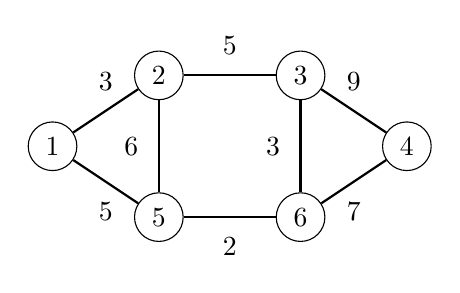
\begin{tikzpicture}[scale=0.9]
\node[draw, circle] (1) at (1.5,2) {$1$};
\node[draw, circle] (2) at (3,3) {$2$};
\node[draw, circle] (3) at (5,3) {$3$};
\node[draw, circle] (4) at (6.5,2) {$4$};
\node[draw, circle] (5) at (3,1) {$5$};
\node[draw, circle] (6) at (5,1) {$6$};
\path[draw,thick,-] (1) -- node[font=\small,label=above:3] {} (2);
\path[draw,thick,-] (2) -- node[font=\small,label=above:5] {} (3);
\path[draw,thick,-] (3) -- node[font=\small,label=above:9] {} (4);
\path[draw,thick,-] (1) -- node[font=\small,label=below:5] {} (5);
\path[draw,thick,-] (5) -- node[font=\small,label=below:2] {} (6);
\path[draw,thick,-] (6) -- node[font=\small,label=below:7] {} (4);
\path[draw,thick,-] (2) -- node[font=\small,label=left:6] {} (5);
\path[draw,thick,-] (3) -- node[font=\small,label=left:3] {} (6);
\end{tikzpicture}
\end{center}
Графтың бір қаңқалы дарағы:
% One spanning tree for the graph is as follows:
\begin{center}
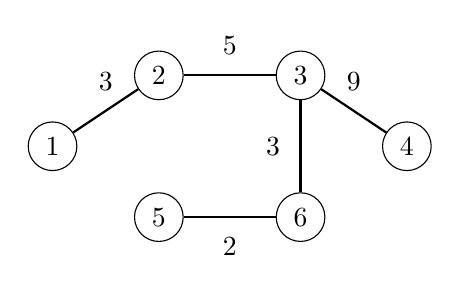
\begin{tikzpicture}[scale=0.9]
\node[draw, circle] (1) at (1.5,2) {$1$};
\node[draw, circle] (2) at (3,3) {$2$};
\node[draw, circle] (3) at (5,3) {$3$};
\node[draw, circle] (4) at (6.5,2) {$4$};
\node[draw, circle] (5) at (3,1) {$5$};
\node[draw, circle] (6) at (5,1) {$6$};
\path[draw,thick,-] (1) -- node[font=\small,label=above:3] {} (2);
\path[draw,thick,-] (2) -- node[font=\small,label=above:5] {} (3);
\path[draw,thick,-] (3) -- node[font=\small,label=above:9] {} (4);
\path[draw,thick,-] (5) -- node[font=\small,label=below:2] {} (6);
\path[draw,thick,-] (3) -- node[font=\small,label=left:3] {} (6);
\end{tikzpicture}
\end{center}

Қаңқалы дарақтың салмағы қыр салмақтарының қосындысына
тең. Мысалы, жоғарыдағы қаңқалы дарақтың салмағы -- $3+5+9+3+2=22$.
% The weight of a spanning tree is the sum of its edge weights.
% For example, the weight of the above spanning tree is
% $3+5+9+3+2=22$.

\index{минималды қаңқалы дарақ}

Минималды қаңқалы дарақ деп салмағы ең аз болатын қаңқалы дарақты айтамыз.
Жоғарыдағы граф үшін минималды қаңқалы дарақтың салмағы 20-ға 
тең болады. Сондай дарақты төмендегідей етіп құрастыруға болады:
% A \key{minimum spanning tree}
% is a spanning tree whose weight is as small as possible.
% The weight of a minimum spanning tree for the example graph
% is 20, and such a tree can be constructed as follows:

\begin{center}
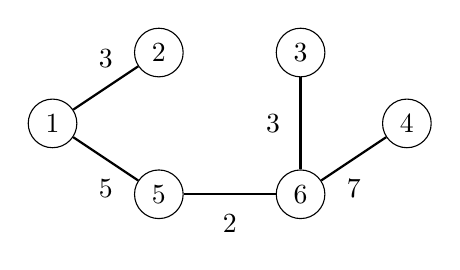
\begin{tikzpicture}[scale=0.9]
\node[draw, circle] (1) at (1.5,2) {$1$};
\node[draw, circle] (2) at (3,3) {$2$};
\node[draw, circle] (3) at (5,3) {$3$};
\node[draw, circle] (4) at (6.5,2) {$4$};
\node[draw, circle] (5) at (3,1) {$5$};
\node[draw, circle] (6) at (5,1) {$6$};

\path[draw,thick,-] (1) -- node[font=\small,label=above:3] {} (2);
\path[draw,thick,-] (1) -- node[font=\small,label=below:5] {} (5);
\path[draw,thick,-] (5) -- node[font=\small,label=below:2] {} (6);
\path[draw,thick,-] (6) -- node[font=\small,label=below:7] {} (4);
\path[draw,thick,-] (3) -- node[font=\small,label=left:3] {} (6);
\end{tikzpicture}
\end{center}

\index{максималды қаңқалы дарақ}

Ұқсас жағдайдағы максималды қаңқалы дарақты алайық. 
Максималды салмақтағы қаңқалы
дарақ максималды қаңқалы дарақ  деп аталады.
Мысалдағы граф үшін максималды қаңқалы дарақтың салмағы 32-ге 
тең болады:
% In a similar way, a \key{maximum spanning tree}
% is a spanning tree whose weight is as large as possible.
% The weight of a maximum spanning tree for the
% example graph is 32:

\begin{center}
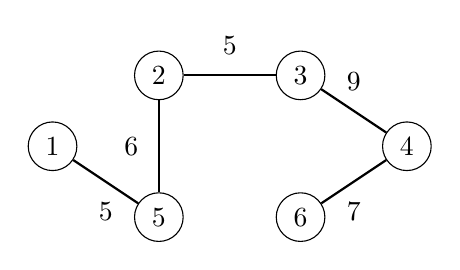
\begin{tikzpicture}[scale=0.9]
\node[draw, circle] (1) at (1.5,2) {$1$};
\node[draw, circle] (2) at (3,3) {$2$};
\node[draw, circle] (3) at (5,3) {$3$};
\node[draw, circle] (4) at (6.5,2) {$4$};
\node[draw, circle] (5) at (3,1) {$5$};
\node[draw, circle] (6) at (5,1) {$6$};
\path[draw,thick,-] (2) -- node[font=\small,label=above:5] {} (3);
\path[draw,thick,-] (3) -- node[font=\small,label=above:9] {} (4);
\path[draw,thick,-] (1) -- node[font=\small,label=below:5] {} (5);
\path[draw,thick,-] (6) -- node[font=\small,label=below:7] {} (4);
\path[draw,thick,-] (2) -- node[font=\small,label=left:6] {} (5);
\end{tikzpicture}
\end{center}

Графта бірнеше минималды және максималды қаңқалы
дарақтың болуы мүмкін екенін ескергеніміз жөн. Сол себепті де дарақ бірегей бола алмайды. 
% Note that a graph may have several
% minimum and maximum spanning trees,
% so the trees are not unique.

Минималды және максималды қаңқалы дарақтарды құру 
үшін бірнеше ашкөз тәсілдерді қолдануға болады.
Бұл бөлімде біз минималды және максималды
қаңқалы дарақтарды құрастыруға көмектесетін 
екі алгоритмді талдаймыз. Екі алгоритм де
графтың қырлары салмағы бойынша реттелген күйде 
жұмыс жасайды. Біз тек минималды қаңқалы дараққа тоқталамыз,
себебі, жай ғана қырлардың ретін ауыстыру арқылы
сол алгоритмдермен максималды қаңқалы дарақ
құруға болады.
% It turns out that several greedy methods
% can be used to construct minimum and maximum
% spanning trees.
% In this chapter, we discuss two algorithms
% that process
% the edges of the graph ordered by their weights.
% We focus on finding minimum spanning trees,
% but the same algorithms can find
% maximum spanning trees by processing the edges in reverse order.

\section{Краскал алгоритмі}

\index{Краскал алгоритмі}

\key{Краскал алгоритміндегі}\footnote{Алгоритмді 1956 жылы Дж.Б.Крускал жариялады \cite{kru56}.} 
алғашқы қаңқалы дарақ ешқандай қыр қамтымай, тек
графтың төбелерінен тұрады. 
Кейін алгоритм қырларды салмағы
бойынша өсу ретімен өтіп шығу барысында
әр қырды қосу немесе қоспау жағдайын тексереді. 
Егер қыр цикл тудырмаса, алгоритм қырды дараққа қосады.

% the initial spanning tree
% only contains the nodes of the graph
% and does not contain any edges.
% Then the algorithm goes through the edges
% ordered by their weights, and always adds an edge
% to the tree if it does not create a cycle.

Алгоритм дарақтың компоненттерін сақтап отырады.
Басында графтың әр төбесі өзі құрап тұрған компонентке
жатады. Кейін қыр жалғанған кезде екі компонент бір-бірімен
қосылады. Нәтижесінде барлық төбелер бір компонентте болады
және минималды қаңқалы дарақ құрылады.
% The algorithm maintains the components
% of the tree.
% Initially, each node of the graph
% belongs to a separate component.
% Always when an edge is added to the tree,
% two components are joined.
% Finally, all nodes belong to the same component,
% and a minimum spanning tree has been found.

\subsubsection{Мысал}

\begin{samepage}
Краскал алгоритмі төмендегі графпен қалай жұмыс жасайтынын
қарастырайық:
% Let us consider how Kruskal's algorithm processes the
% following graph:
\begin{center}
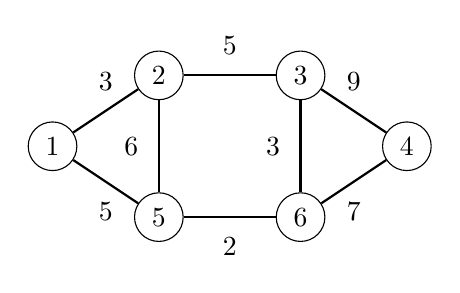
\begin{tikzpicture}[scale=0.9]
\node[draw, circle] (1) at (1.5,2) {$1$};
\node[draw, circle] (2) at (3,3) {$2$};
\node[draw, circle] (3) at (5,3) {$3$};
\node[draw, circle] (4) at (6.5,2) {$4$};
\node[draw, circle] (5) at (3,1) {$5$};
\node[draw, circle] (6) at (5,1) {$6$};
\path[draw,thick,-] (1) -- node[font=\small,label=above:3] {} (2);
\path[draw,thick,-] (2) -- node[font=\small,label=above:5] {} (3);
\path[draw,thick,-] (3) -- node[font=\small,label=above:9] {} (4);
\path[draw,thick,-] (1) -- node[font=\small,label=below:5] {} (5);
\path[draw,thick,-] (5) -- node[font=\small,label=below:2] {} (6);
\path[draw,thick,-] (6) -- node[font=\small,label=below:7] {} (4);
\path[draw,thick,-] (2) -- node[font=\small,label=left:6] {} (5);
\path[draw,thick,-] (3) -- node[font=\small,label=left:3] {} (6);
\end{tikzpicture}
\end{center}
\end{samepage}

\begin{samepage}
Алгоритмнің бірінші қадамы -- қырларды өсу ретінде реттеу.
Оның нәтижесі:
% The first step of the algorithm is to sort the
% edges in increasing order of their weights.
% The result is the following list:

\begin{tabular}{ll}
\\
қыр & салмағы \\
\hline
5--6 & 2 \\
1--2 & 3 \\
3--6 & 3 \\
1--5 & 5 \\
2--3 & 5 \\
2--5 & 6 \\
4--6 & 7 \\
3--4 & 9 \\
\\
\end{tabular}
\end{samepage}

Осыдан кейін алгоритм тізім арқылы өтіп, 
егер қыр екі бөлек компонентті біріктірсе, ол қырды 
дараққа қосады.
% After this, the algorithm goes through the list
% and adds each edge to the tree if it joins
% two separate components.

Бастапқыда әр төбе өзі құрап тұрған компоненттен тұрады: 
% Initially, each node is in its own component:

\begin{center}
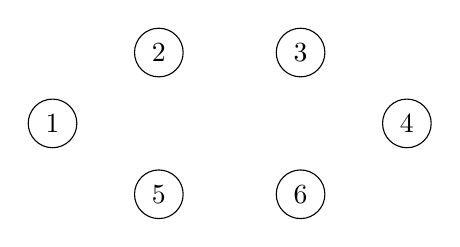
\begin{tikzpicture}[scale=0.9]
\node[draw, circle] (1) at (1.5,2) {$1$};
\node[draw, circle] (2) at (3,3) {$2$};
\node[draw, circle] (3) at (5,3) {$3$};
\node[draw, circle] (4) at (6.5,2) {$4$};
\node[draw, circle] (5) at (3,1) {$5$};
\node[draw, circle] (6) at (5,1) {$6$};
%\path[draw,thick,-] (1) -- node[font=\small,label=above:3] {} (2);
%\path[draw,thick,-] (2) -- node[font=\small,label=above:5] {} (3);
%\path[draw,thick,-] (3) -- node[font=\small,label=above:9] {} (4);
%\path[draw,thick,-] (1) -- node[font=\small,label=below:5] {} (5);
%\path[draw,thick,-] (5) -- node[font=\small,label=below:2] {} (6);
%\path[draw,thick,-] (6) -- node[font=\small,label=below:7] {} (4);
%\path[draw,thick,-] (2) -- node[font=\small,label=left:6] {} (5);
%\path[draw,thick,-] (3) -- node[font=\small,label=left:3] {} (6);
\end{tikzpicture}
\end{center}
Дараққа қосылатын бірінші қыр -- 5--6. Осы 
$\{5\}$ пен $\{6\}$ қырлардың компоненттерін қосу арқылы 
біртұтас $\{5,6\}$ компоненті құрылды.
% The first edge to be added to the tree is
% the edge 5--6 that creates a component $\{5,6\}$
% by joining the components $\{5\}$ and $\{6\}$:

\begin{center}
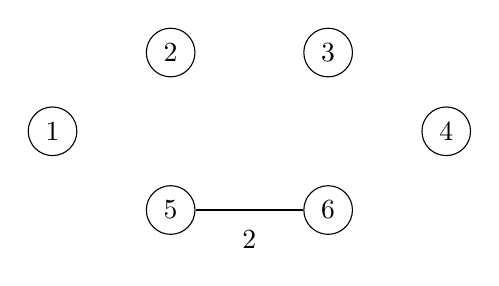
\begin{tikzpicture}
\node[draw, circle] (1) at (1.5,2) {$1$};
\node[draw, circle] (2) at (3,3) {$2$};
\node[draw, circle] (3) at (5,3) {$3$};
\node[draw, circle] (4) at (6.5,2) {$4$};
\node[draw, circle] (5) at (3,1) {$5$};
\node[draw, circle] (6) at (5,1) {$6$};

%\path[draw,thick,-] (1) -- node[font=\small,label=above:3] {} (2);
%\path[draw,thick,-] (2) -- node[font=\small,label=above:5] {} (3);
%\path[draw,thick,-] (3) -- node[font=\small,label=above:9] {} (4);
%\path[draw,thick,-] (1) -- node[font=\small,label=below:5] {} (5);
\path[draw,thick,-] (5) -- node[font=\small,label=below:2] {} (6);
%\path[draw,thick,-] (6) -- node[font=\small,label=below:7] {} (4);
%\path[draw,thick,-] (2) -- node[font=\small,label=left:6] {} (5);
%\path[draw,thick,-] (3) -- node[font=\small,label=left:3] {} (6);
\end{tikzpicture}
\end{center}
Содан кейін 1--2, 3--6 және 1--5 қырлары ұқсас әдіспен қосылады:
% After this, the edges 1--2, 3--6 and 1--5 are added in a similar way:

\begin{center}
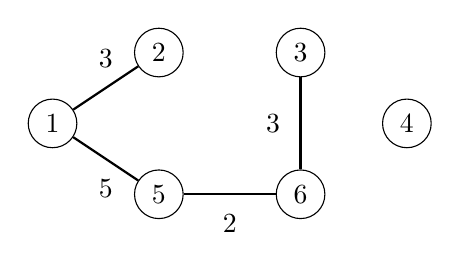
\begin{tikzpicture}[scale=0.9]
\node[draw, circle] (1) at (1.5,2) {$1$};
\node[draw, circle] (2) at (3,3) {$2$};
\node[draw, circle] (3) at (5,3) {$3$};
\node[draw, circle] (4) at (6.5,2) {$4$};
\node[draw, circle] (5) at (3,1) {$5$};
\node[draw, circle] (6) at (5,1) {$6$};

\path[draw,thick,-] (1) -- node[font=\small,label=above:3] {} (2);
%\path[draw,thick,-] (2) -- node[font=\small,label=above:5] {} (3);
%\path[draw,thick,-] (3) -- node[font=\small,label=above:9] {} (4);
\path[draw,thick,-] (1) -- node[font=\small,label=below:5] {} (5);
\path[draw,thick,-] (5) -- node[font=\small,label=below:2] {} (6);
%\path[draw,thick,-] (6) -- node[font=\small,label=below:7] {} (4);
%\path[draw,thick,-] (2) -- node[font=\small,label=left:6] {} (5);
\path[draw,thick,-] (3) -- node[font=\small,label=left:3] {} (6);
\end{tikzpicture}
\end{center}

Бұл қадамдардан кейін  компоненттердің көбі біріктіріледі де
дарақта тек екі компонент қалады:
$\{1,2,3,5,6\}$ және $\{4\}$.
% After those steps, most components have been joined
% and there are two components in the tree:
% $\{1,2,3,5,6\}$ and $\{4\}$.

Тізімдегі келесі қыр -- 2--3 қыры. Бірақ ол
дараққа қосылмайды. Себебі 2 және 3 төбелері әлдеқашан
компонентке біріктірілген.
Дәл осы себеппен 2--5 қыры да дараққа қосылмайды.
% The next edge in the list is the edge 2--3,
% but it will not be included in the tree, because
% nodes 2 and 3 are already in the same component.
% For the same reason, the edge 2--5 will not be included in the tree.

\begin{samepage}
Соңында 4--6 қыры дараққа қосылады:
% Finally, the edge 4--6 will be included in the tree:

\begin{center}
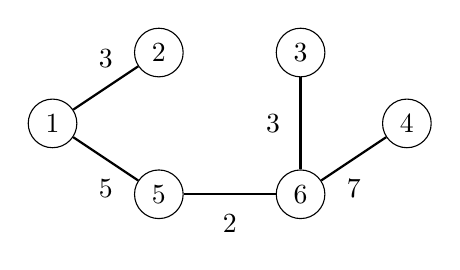
\begin{tikzpicture}[scale=0.9]
\node[draw, circle] (1) at (1.5,2) {$1$};
\node[draw, circle] (2) at (3,3) {$2$};
\node[draw, circle] (3) at (5,3) {$3$};
\node[draw, circle] (4) at (6.5,2) {$4$};
\node[draw, circle] (5) at (3,1) {$5$};
\node[draw, circle] (6) at (5,1) {$6$};

\path[draw,thick,-] (1) -- node[font=\small,label=above:3] {} (2);
%\path[draw,thick,-] (2) -- node[font=\small,label=above:5] {} (3);
%\path[draw,thick,-] (3) -- node[font=\small,label=above:9] {} (4);
\path[draw,thick,-] (1) -- node[font=\small,label=below:5] {} (5);
\path[draw,thick,-] (5) -- node[font=\small,label=below:2] {} (6);
\path[draw,thick,-] (6) -- node[font=\small,label=below:7] {} (4);
%\path[draw,thick,-] (2) -- node[font=\small,label=left:6] {} (5);
\path[draw,thick,-] (3) -- node[font=\small,label=left:3] {} (6);
\end{tikzpicture}
\end{center}
\end{samepage}

Бұдан кейін
алгоритм ешқандай қыр қоспайды. Өйткені граф толық байланысып тұр.
Соңғы құрастырылған граф -- салмағы $2+3+3+5+7=20$ тең
минималды қаңқалы дарақ.
% After this, the algorithm will not add any
% new edges, because the graph is connected
% and there is a path between any two nodes.
% The resulting graph is a minimum spanning tree
% with weight $2+3+3+5+7=20$.

\subsubsection{Жұмыс істеу себебі неде?}
%here
''Краскал алгоритмі қалай жұмыс істейді? 
Ашкөз стратегиясы неліктен минималды қаңқалы дарақты
табуға кепілдік береді?'' - деген жақсы сұрақ туындайды.
% It is a good question why Kruskal's algorithm works.
% Why does the greedy strategy guarantee that we
% will find a minimum spanning tree?

Графтың ең аз салмақты қыры қаңқалы
дараққа \emph{қосылмаса} не болатынын бақылап көрейік.
Мысалы, төменде берілген графтың қаңқалы дарағы
5--6 қырын қамтымады деп есептейік.
Біз дарақтың дәл құрылымын білмейміз. Бірақ
ол қандай да бір қырларды қамтуы қажет.
Дарақ келесідей болады делік:

% Let us see what happens if the minimum weight edge of
% the graph is \emph{not} included in the spanning tree.
% For example, suppose that a spanning tree
% for the previous graph would not contain the
% minimum weight edge 5--6.
% We do not know the exact structure of such a spanning tree,
% but in any case it has to contain some edges.
% Assume that the tree would be as follows:

\begin{center}
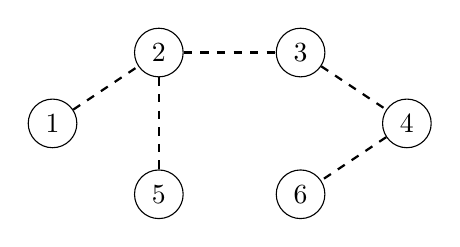
\begin{tikzpicture}[scale=0.9]
\node[draw, circle] (1) at (1.5,2) {$1$};
\node[draw, circle] (2) at (3,3) {$2$};
\node[draw, circle] (3) at (5,3) {$3$};
\node[draw, circle] (4) at (6.5,2) {$4$};
\node[draw, circle] (5) at (3,1) {$5$};
\node[draw, circle] (6) at (5,1) {$6$};

\path[draw,thick,-,dashed] (1) -- (2);
\path[draw,thick,-,dashed] (2) -- (5);
\path[draw,thick,-,dashed] (2) -- (3);
\path[draw,thick,-,dashed] (3) -- (4);
\path[draw,thick,-,dashed] (4) -- (6);
\end{tikzpicture}
\end{center}

Бірақ жоғарыда көрсетілген суреттегі қаңқалы дарақ минималды бола алмайды, өйткені бізге одан қандай да бір қырды алып тастауға және оны минималды салмағы 5--6 болатын қырмен ауыстыруға ешнәрсе кедергі келтірмейді.
Осылайша салмағы \emph{азырақ} қаңқалы дарақ құралады:
% However, it is not possible that the above tree
% would be a minimum spanning tree for the graph.
% The reason for this is that we can remove an edge
% from the tree and replace it with the minimum weight edge 5--6.
% This produces a spanning tree whose weight is
% \emph{smaller}:

\begin{center}
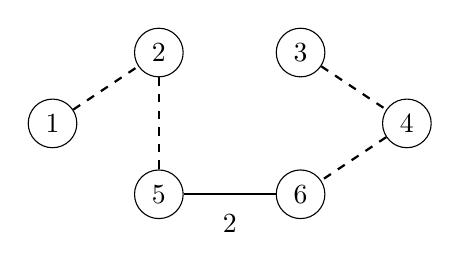
\begin{tikzpicture}[scale=0.9]
\node[draw, circle] (1) at (1.5,2) {$1$};
\node[draw, circle] (2) at (3,3) {$2$};
\node[draw, circle] (3) at (5,3) {$3$};
\node[draw, circle] (4) at (6.5,2) {$4$};
\node[draw, circle] (5) at (3,1) {$5$};
\node[draw, circle] (6) at (5,1) {$6$};

\path[draw,thick,-,dashed] (1) -- (2);
\path[draw,thick,-,dashed] (2) -- (5);
\path[draw,thick,-,dashed] (3) -- (4);
\path[draw,thick,-,dashed] (4) -- (6);
\path[draw,thick,-] (5) -- node[font=\small,label=below:2] {} (6);
\end{tikzpicture}
\end{center}

Сол себепті салмағы ең аз қаңқалы дарақты құру үшін
дараққа ең аз салмақты қырларды қосу әрқашан оңтайлы.
Ұқсас пайымдауды қолдана отырып,   келесі минималды салмағы бар және т.с.с. қырды қосу қажет екенін көрсетуге болады. Сондықтан Краскал алгоритмі әрқашан минималды қаңқалы дарақты береді.
% For this reason, it is always optimal
% to include the minimum weight edge
% in the tree to produce a minimum spanning tree.
% Using a similar argument, we can show that it
% is also optimal to add the next edge in weight order
% to the tree, and so on.
% Hence, Kruskal's algorithm works correctly and
% always produces a minimum spanning tree.

\subsubsection{Кодтың жазылуы}

Краскал алгоритмінің кодын жазған кезде қырлар тізімі
көрінісін қолдану қолайлырақ. Алгоритмнің бірінші 
бөлігі тізімдегі қырларды $O(m \log m)$ уақытында реттейді.
Осыдан кейін төменде көрсетілгендей алгоритмнің екінші бөлігінде 
ең аз қаңқалы дарақ құрылады:
% When implementing Kruskal's algorithm,
% it is convenient to use
% the edge list representation of the graph.
% The first phase of the algorithm sorts the
% edges in the list in $O(m \log m)$ time.
% After this, the second phase of the algorithm
% builds the minimum spanning tree as follows:

\begin{lstlisting}
for (...) {
  if (!same(a,b)) unite(a,b);
}
\end{lstlisting}

Цикл тізімдегі қырларды өтіп шығады және $a$ мен $b$ төбелерін қосатын әрбір $a$--$b$
қырларын өңдейді.
Алгоритмді жүзеге асыру үшін екі 
функция қажет. Олар: $a$ және 
$b$ бір компонентте екенін анықтайтын \texttt{same} функциясы және $a$ және $b$ компоненттерін біріктіретін \texttt{unite}
функциясы.
% The loop goes through the edges in the list
% and always processes an edge $a$--$b$
% where $a$ and $b$ are two nodes.
% Two functions are needed:
% the function \texttt{same} determines
% if $a$ and $b$ are in the same component,
% and the function \texttt{unite}
% joins the components that contain $a$ and $b$.

Әңгіме \texttt{same} және \texttt{unite} функцияларын 
қалай тиімді іске асыруға болады деген мәселеге барып тіреледі. Оның бір жолы -- графты аралау арқылы  \texttt{same} функциясын жүзеге асыру. Бұл кезде алгоритм $a$ төбесінен $b$ төбесіне өту 
мүмкіндігін тереңдік бойынша ізденіспен тексереді. 
Дегенмен мұндай функцияның уақытша күрделілігі -- $O(n+m)$.
Сондықтан алгоритм баяу болады. Өйткені \texttt{same} функциясы
графтың әр қыры үшін шақырылады.
% The problem is how to efficiently implement
% the functions \texttt{same} and \texttt{unite}.
% One possibility is to implement the function
% \texttt{same} as a graph traversal and check if
% we can get from node $a$ to node $b$.
% However, the time complexity of such a function
% would be $O(n+m)$
% and the resulting algorithm would be slow,
% because the function \texttt{same} will be called for each edge in the graph.

Біз есепті қиылыспайтын жиындар құрылымының -- $O(\log n)$ уақытта екі функцияны да жүзеге асыруға мүмкіндік беретін деректер құрылымының көмегімен шешеміз. Осылайша, қырлар тізімін сұрыптап болғаннан кейінгі
Краскал алгоритмінің уақытша күрделілігі $O(m \log n)$ болмақ.
% We will solve the problem using a union-find structure
% that implements both functions in $O(\log n)$ time.
% Thus, the time complexity of Kruskal's algorithm
% will be $O(m \log n)$ after sorting the edge list.

\section{Қиылыспайтын жиындар құрылымы}

\index{қиылыспайтын жиындар құрылымы}

Қиылыспайтын жиындар құрылымы (union-find structure) жиындар топтамасынан
тұрады. Бұл жиындар екеуара қиылыспайды, яғни әр элемент бір жиынға ғана кіреді.
Қиылыспайтын жиындар құрылымы
уақытша күрделілігі $O(\log n)$ болатын екі амалды қолдайды. Олар: екі жиынды біріктіретін
\texttt{unite} амалы және берілген элементті құрайтын жиынның басшысын табатын 
\texttt{find} амалы\footnote{Ұсынылған құрылымды 1971 жылы Дж. Д. Хопкрофт пен Дж. Д. Ульман енгізген болатын \cite{hop71}.
Ал 1975 жылы Р.Е.Тарьян бүгінде көптеген оқулықтарда талқыланып жүрген алгоритм құрылымының күрделі нұсқасын зерттеді \cite{tar75}.}.
% a collection of sets.
% The sets are disjoint, so no element
% belongs to more than one set.
% Two $O(\log n)$ time operations are supported:
% the \texttt{unite} operation joins two sets,
% and the \texttt{find} operation finds the representative
% of the set that contains a given element\footnote{The structure presented here
% was introduced in 1971 by J. D. Hopcroft and J. D. Ullman \cite{hop71}.
% Later, in 1975, R. E. Tarjan studied a more sophisticated variant
% of the structure \cite{tar75} that is discussed in many algorithm
% textbooks nowadays.}.

\subsubsection{Құрылым}
%--------------------------------------------------
Қиылыспайтын жиындар құрылымындағы әр жиында бір элемент
басшы болады және жиынның кез келген элементінен оның басшысына қарай жол түседі. 
Мысалы, $\{1,4,7\}$, $\{5\}$ және $\{2,3,6,8\}$ жиындарын 
төмендегі ретпен қарастырып көрейік:
% In a union-find structure, one element in each set
% is the representative of the set,
% and there is a chain from any other element of the
% set to the representative.
% For example, assume that the sets are
% $\{1,4,7\}$, $\{5\}$ and $\{2,3,6,8\}$:
\begin{center}
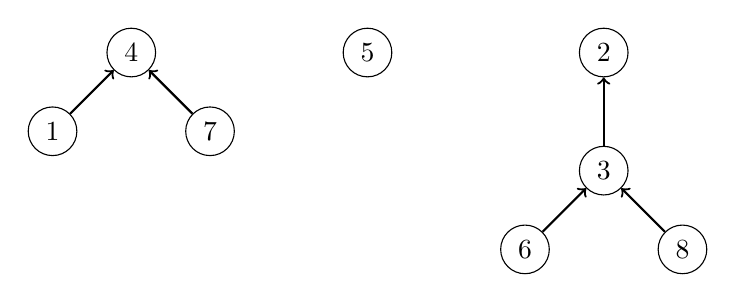
\begin{tikzpicture}
\node[draw, circle] (1) at (0,-1) {$1$};
\node[draw, circle] (2) at (7,0) {$2$};
\node[draw, circle] (3) at (7,-1.5) {$3$};
\node[draw, circle] (4) at (1,0) {$4$};
\node[draw, circle] (5) at (4,0) {$5$};
\node[draw, circle] (6) at (6,-2.5) {$6$};
\node[draw, circle] (7) at (2,-1) {$7$};
\node[draw, circle] (8) at (8,-2.5) {$8$};

\path[draw,thick,->] (1) -- (4);
\path[draw,thick,->] (7) -- (4);

\path[draw,thick,->] (3) -- (2);
\path[draw,thick,->] (6) -- (3);
\path[draw,thick,->] (8) -- (3);

\end{tikzpicture}
\end{center}
Мұндағы  4, 5 және 2 -- жиындардың басшылары болып саналады.
Кез келген элементтің басшысын табу үшін сол элементтен басталатын жолмен өтіп шығу керек. 
Мысалы, 2-элемент 6-элементінің басшысы, себебі біз
$6 \rightarrow 3 \rightarrow 2$ тізбегімен жүріп, 2-элементте
тоқтадық.
Басшылары бір болса ғана екі элемент бір жиынға жатады.
% In this case the representatives
% of the sets are 4, 5 and 2.
% We can find the representative of any element
% by following the chain that begins at the element.
% For example, the element 2 is the representative
% for the element 6, because
% we follow the chain $6 \rightarrow 3 \rightarrow 2$.
% Two elements belong to the same set exactly when
% their representatives are the same.

Бір жиынның басшысын екінші жиынның басшысына 
жалғау арқылы екі жиынды қосуға болады.
% Two sets can be joined by connecting the
% representative of one set to the
% representative of the other set.
Мысалы, $\{1,4,7\}$ және $\{2,3,6,8\}$ жиындарын
келесі ретпен қосуға болады:
% For example, the sets
% $\{1,4,7\}$ and $\{2,3,6,8\}$
% can be joined as follows:
\begin{center}
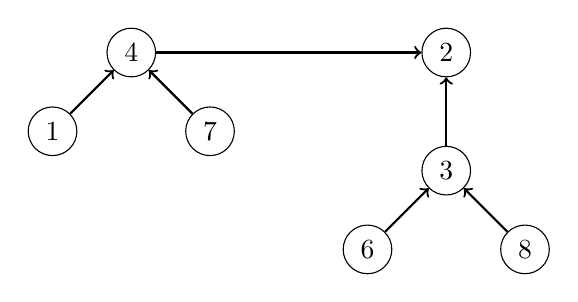
\begin{tikzpicture}
\node[draw, circle] (1) at (2,-1) {$1$};
\node[draw, circle] (2) at (7,0) {$2$};
\node[draw, circle] (3) at (7,-1.5) {$3$};
\node[draw, circle] (4) at (3,0) {$4$};
\node[draw, circle] (6) at (6,-2.5) {$6$};
\node[draw, circle] (7) at (4,-1) {$7$};
\node[draw, circle] (8) at (8,-2.5) {$8$};

\path[draw,thick,->] (1) -- (4);
\path[draw,thick,->] (7) -- (4);

\path[draw,thick,->] (3) -- (2);
\path[draw,thick,->] (6) -- (3);
\path[draw,thick,->] (8) -- (3);

\path[draw,thick,->] (4) -- (2);
\end{tikzpicture}
\end{center}

Одан шығатын жиын $\{1,2,3,4,6,7,8\}$
элементтерін қамтиды.
% The resulting set contains the elements
% $\{1,2,3,4,6,7,8\}$.
Кейін 2-элемент екі жиынның басшысы болады және
бұрынғы басшы 4 енді 2-элементке нұсқайды.
% From this on, the element 2 is the representative
% for the entire set and the old representative 4
% points to the element 2.

Қиылыспайтын жиындар құрылымының тиімділігі жиындардың қалай біріктірілгеніне байланысты болады. Біз қарапайым стратегияны пайдалана аламыз, яғни әрқашан кіші жиынның басшысын үлкен жиынның басшысына қосамыз (ал егер  
жиындардың мөлшері бірдей болса, ерікті таңдау жасаймыз).
Мұндай стратегияда кез келген жолдың ұзындығы 
$O(\log n)$ болады. Сондықтан біз сәйкес жолмен жүру арқылы кез келген элементтің басшысын оңтайлы таба аламыз.
% The efficiency of the union-find structure depends on
% how the sets are joined.
% It turns out that we can follow a simple strategy:
% always connect the representative of the
% \emph{smaller} set to the representative of the \emph{larger} set
% (or if the sets are of equal size,
% we can make an arbitrary choice).
% Using this strategy, the length of any chain
% will be $O(\log n)$, so we can
% find the representative of any element
% efficiently by following the corresponding chain.

\subsubsection{Кодтың жазылуы}

Қиылыспайтын жиындар құрылымының кодын жиымдар арқылы
жазуға болады. Келесі кодта \texttt{link} жиымы
тізбектегі әр элемент үшін келесі элементті, ал
басшы болса өзін сақтайды. Сондай-ақ \texttt{size} жиымы
әр басшы үшін сәйкес жиынының мөлшерін көрсетеді.

% The union-find structure can be implemented
% using arrays.
% In the following implementation,
% the array \texttt{link} contains for each element
% the next element
% in the chain or the element itself if it is
% a representative,
% and the array \texttt{size} indicates for each representative
% the size of the corresponding set.

Басында, әр элемент жеке жиынға жатады:
\begin{lstlisting}
for (int i = 1; i <= n; i++) link[i] = i;
for (int i = 1; i <= n; i++) size[i] = 1;
\end{lstlisting}

\texttt{find} функциясы $x$-элементтің
басшысын тауып береді.
Басшыны $x$ элементінен басталатын жолдың 
бойымен жүру арқылы табуға болады.
% The function \texttt{find} returns
% the representative for an element $x$.
% The representative can be found by following
% the chain that begins at $x$.

\begin{lstlisting}
int find(int x) {
    while (x != link[x]) x = link[x];
    return x;
}
\end{lstlisting}

\texttt{same} функциясы $a$ мен $b$ элементтері бір 
жиынға жататындығын тексереді. Мұны \texttt{find}
функциясы арқылы оңай тексеруге болады:
% The function \texttt{same} checks
% whether elements $a$ and $b$ belong to the same set.
% This can easily be done by using the
% function \texttt{find}:

\begin{lstlisting}
bool same(int a, int b) {
    return find(a) == find(b);
}
\end{lstlisting}

\begin{samepage}
\texttt{unite} функциясы $a$ және $b$ элементтерін
қамтитын жиындарды біріктіреді (осы екі элемент әртүрлі
жиында болуы қажет). Функция бірінші жиынның басшысын табады,
кейін кіші жиынды үлкен жиынға қосады.
% The function \texttt{unite} joins the sets
% that contain elements $a$ and $b$
% (the elements have to be in different sets).
% The function first finds the representatives
% of the sets and then connects the smaller
% set to the larger set.

\begin{lstlisting}
void unite(int a, int b) {
    a = find(a);
    b = find(b);
    if (size[a] < size[b]) swap(a,b);
    size[a] += size[b];
    link[b] = a;
}
\end{lstlisting}
\end{samepage}

Әр тізбектің ұзындығы $O(\log n)$ болса, 
\texttt{find} функциясының уақытша күрделілігі $O(\log n)$-ге тең.
Осы жағдайда \texttt{same} мен \texttt{unite} функциялары
$O(\log n)$ уақытында жұмыс жасайды.
\texttt{unite} функциясы кіші жиынды үлкен жиынға қосу арқылы
жол тізбегін $O(\log n)$ ұзындығынан асырмауға тырысады.
% The time complexity of the function \texttt{find}
% is $O(\log n)$ assuming that the length of each
% chain is $O(\log n)$.
% In this case, the functions \texttt{same} and \texttt{unite}
% also work in $O(\log n)$ time.
% The function \texttt{unite} makes sure that the
% length of each chain is $O(\log n)$ by connecting
% the smaller set to the larger set.

\section{Прим алгоритмі}

\index{Прим алгоритмі}

\key{Прим алгоритмі}\footnote{Алгоритм оны 1957 жылы жариялаған Р.С.Примнің атымен аталған \cite{pri57}.
Дегенмен дәл осындай алгоритмді 1930 жылы В.Ярник ашқан болатын.} 
минималды қаңқалы дарақты табудың балама әдісіне жатады.
Алдымен ол дараққа еркін төбені қосады.
Ал келесі төбелерді қосу барысында минималды салмағы бар қырды таңдайды. Барлық төбелер қосылғаннан кейін, минималды қаңқалы дарақ құрылады.
% The algorithm first adds an arbitrary node
% to the tree.
% After this, the algorithm always chooses
% a minimum-weight edge that
% adds a new node to the tree.
% Finally, all nodes have been added to the tree
% and a minimum spanning tree has been found.

Прим алгоритмі Дейкстра алгоритміне ұқсас болып келеді.
Бірақ, олардың аздаған айырмашылығы бар: Дейкстра алгоритмі әрқашан
бастапқы төбеден арақашықтығы ең аз болатындай қырды таңдаса, Прим
алгоритмі қарапайым дараққа жаңа төбені қосатын ең аз қырды таңдайды.

% Prim's algorithm resembles Dijkstra's algorithm.
% The difference is that Dijkstra's algorithm always
% selects an edge whose distance from the starting
% node is minimum, but Prim's algorithm simply selects
% the minimum weight edge that adds a new node to the tree.

\subsubsection{Мысал}

Прим алгоритмі төмендегі графта қалай жұмыс істейтінін қарастырайық:

\begin{center}
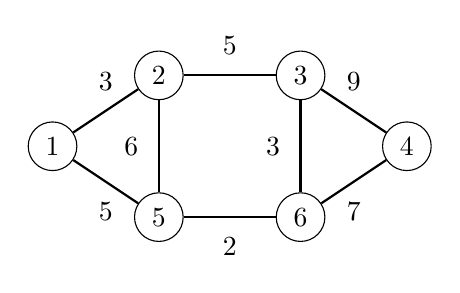
\begin{tikzpicture}[scale=0.9]
\node[draw, circle] (1) at (1.5,2) {$1$};
\node[draw, circle] (2) at (3,3) {$2$};
\node[draw, circle] (3) at (5,3) {$3$};
\node[draw, circle] (4) at (6.5,2) {$4$};
\node[draw, circle] (5) at (3,1) {$5$};
\node[draw, circle] (6) at (5,1) {$6$};
\path[draw,thick,-] (1) -- node[font=\small,label=above:3] {} (2);
\path[draw,thick,-] (2) -- node[font=\small,label=above:5] {} (3);
\path[draw,thick,-] (3) -- node[font=\small,label=above:9] {} (4);
\path[draw,thick,-] (1) -- node[font=\small,label=below:5] {} (5);
\path[draw,thick,-] (5) -- node[font=\small,label=below:2] {} (6);
\path[draw,thick,-] (6) -- node[font=\small,label=below:7] {} (4);
\path[draw,thick,-] (2) -- node[font=\small,label=left:6] {} (5);
\path[draw,thick,-] (3) -- node[font=\small,label=left:3] {} (6);

%\path[draw=red,thick,-,line width=2pt] (5) -- (6);
\end{tikzpicture}
\end{center}
Бастапқыда төбелер арасында ешқандай қыр болмайды:
\begin{center}
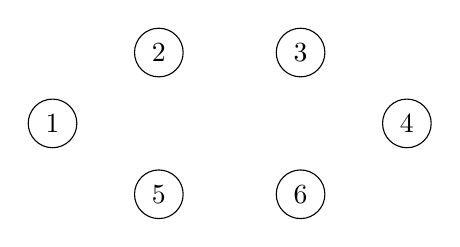
\begin{tikzpicture}[scale=0.9]
\node[draw, circle] (1) at (1.5,2) {$1$};
\node[draw, circle] (2) at (3,3) {$2$};
\node[draw, circle] (3) at (5,3) {$3$};
\node[draw, circle] (4) at (6.5,2) {$4$};
\node[draw, circle] (5) at (3,1) {$5$};
\node[draw, circle] (6) at (5,1) {$6$};
%\path[draw,thick,-] (1) -- node[font=\small,label=above:3] {} (2);
%\path[draw,thick,-] (2) -- node[font=\small,label=above:5] {} (3);
%\path[draw,thick,-] (3) -- node[font=\small,label=above:9] {} (4);
%\path[draw,thick,-] (1) -- node[font=\small,label=below:5] {} (5);
%\path[draw,thick,-] (5) -- node[font=\small,label=below:2] {} (6);
%\path[draw,thick,-] (6) -- node[font=\small,label=below:7] {} (4);
%\path[draw,thick,-] (2) -- node[font=\small,label=left:6] {} (5);
%\path[draw,thick,-] (3) -- node[font=\small,label=left:3] {} (6);
\end{tikzpicture}
\end{center}
Еркін төбе ретінде 1-төбені таңдайық.
Алдымен біз салмағы 3-ке тең қыр арқылы 2-төбені қосамыз:
% An arbitrary node can be the starting node,
% so let us choose node 1.
% First, we add node 2 that is connected by
% an edge of weight 3:
\begin{center}
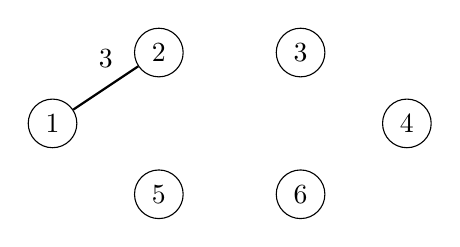
\begin{tikzpicture}[scale=0.9]
\node[draw, circle] (1) at (1.5,2) {$1$};
\node[draw, circle] (2) at (3,3) {$2$};
\node[draw, circle] (3) at (5,3) {$3$};
\node[draw, circle] (4) at (6.5,2) {$4$};
\node[draw, circle] (5) at (3,1) {$5$};
\node[draw, circle] (6) at (5,1) {$6$};
\path[draw,thick,-] (1) -- node[font=\small,label=above:3] {} (2);
%\path[draw,thick,-] (2) -- node[font=\small,label=above:5] {} (3);
%\path[draw,thick,-] (3) -- node[font=\small,label=above:9] {} (4);
%\path[draw,thick,-] (1) -- node[font=\small,label=below:5] {} (5);
%\path[draw,thick,-] (5) -- node[font=\small,label=below:2] {} (6);
%\path[draw,thick,-] (6) -- node[font=\small,label=below:7] {} (4);
%\path[draw,thick,-] (2) -- node[font=\small,label=left:6] {} (5);
%\path[draw,thick,-] (3) -- node[font=\small,label=left:3] {} (6);
\end{tikzpicture}
\end{center}

Бұдан кейін салмағы 5-ке тең екі қыр қалады. Сол себепті біз дараққа не 3-төбені, не 5-төбені қосуға мүмкіндік аламыз.
Алдымен 3-төбені қосып көрейік:
% After this, there are two edges with weight 5,
% so we can add either node 3 or node 5 to the tree.
% Let us add node 3 first:
\begin{center}
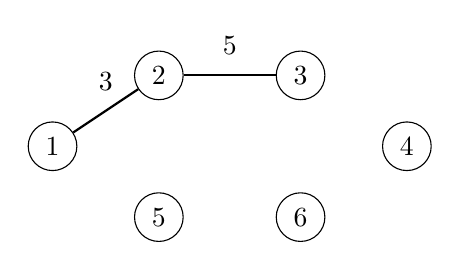
\begin{tikzpicture}[scale=0.9]
\node[draw, circle] (1) at (1.5,2) {$1$};
\node[draw, circle] (2) at (3,3) {$2$};
\node[draw, circle] (3) at (5,3) {$3$};
\node[draw, circle] (4) at (6.5,2) {$4$};
\node[draw, circle] (5) at (3,1) {$5$};
\node[draw, circle] (6) at (5,1) {$6$};
\path[draw,thick,-] (1) -- node[font=\small,label=above:3] {} (2);
\path[draw,thick,-] (2) -- node[font=\small,label=above:5] {} (3);
%\path[draw,thick,-] (3) -- node[font=\small,label=above:9] {} (4);
%\path[draw,thick,-] (1) -- node[font=\small,label=below:5] {} (5);
%\path[draw,thick,-] (5) -- node[font=\small,label=below:2] {} (6);
%\path[draw,thick,-] (6) -- node[font=\small,label=below:7] {} (4);
%\path[draw,thick,-] (2) -- node[font=\small,label=left:6] {} (5);
%\path[draw,thick,-] (3) -- node[font=\small,label=left:3] {} (6);
\end{tikzpicture}
\end{center}

\begin{samepage}
Осы процесс барлық төбелер дараққа қосылғанша жалғасады: 
% The process continues until all nodes have been included in the tree:
\begin{center}
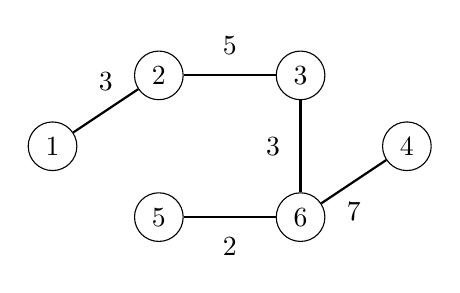
\begin{tikzpicture}[scale=0.9]
\node[draw, circle] (1) at (1.5,2) {$1$};
\node[draw, circle] (2) at (3,3) {$2$};
\node[draw, circle] (3) at (5,3) {$3$};
\node[draw, circle] (4) at (6.5,2) {$4$};
\node[draw, circle] (5) at (3,1) {$5$};
\node[draw, circle] (6) at (5,1) {$6$};
\path[draw,thick,-] (1) -- node[font=\small,label=above:3] {} (2);
\path[draw,thick,-] (2) -- node[font=\small,label=above:5] {} (3);
%\path[draw,thick,-] (3) -- node[font=\small,label=above:9] {} (4);
%\path[draw,thick,-] (1) -- node[font=\small,label=below:5] {} (5);
\path[draw,thick,-] (5) -- node[font=\small,label=below:2] {} (6);
\path[draw,thick,-] (6) -- node[font=\small,label=below:7] {} (4);
%\path[draw,thick,-] (2) -- node[font=\small,label=left:6] {} (5);
\path[draw,thick,-] (3) -- node[font=\small,label=left:3] {} (6);
\end{tikzpicture}
\end{center}
\end{samepage}

\subsubsection{Кодтың жазылуы}

Дейкстра алгоритмі сияқты Прим алгоритмін де басымдылық кезегін қолдана
отырып, тиімді жазуға болады. Басымдылық кезегі қазіргі компонентке
бір қырмен қосуға болатын барлық төбелерді сақтауы керек. Бұл жерде 
Дейкстра алгоритміндегідей төбелерді салмағының өсу ретімен сақтайды.

% Like Dijkstra's algorithm, Prim's algorithm can be
% efficiently implemented using a priority queue.
% The priority queue should contain all nodes
% that can be connected to the current component using
% a single edge, in increasing order of the weights
% of the corresponding edges.

Прим алгоритмінің уақытша күрделілігі Дейкстра алгоритміндегідей
$O(n + m \log m)$ болады. Көбінесе Примнің және Краскалдың 
алгоритмдері бірдей тиімді. Сондықтан қай алгоритмді таңдау мәселесі әр адамның
қалауына байланысты болмақ.
Дегенмен спорттық бағдарламалаушылардың көпшілігі Крускал алгоритмін пайдаланады.
% The time complexity of Prim's algorithm is
% $O(n + m \log m)$ that equals the time complexity
% of Dijkstra's algorithm.
% In practice, Prim's and Kruskal's algorithms
% are both efficient, and the choice of the algorithm
% is a matter of taste.
% Still, most competitive programmers use Kruskal's algorithm.